\documentclass{article}

\usepackage{fancyhdr}
\usepackage{extramarks}
\usepackage{amsmath}
\usepackage{amsthm}
\usepackage{amsfonts}
\usepackage{amssymb}
\usepackage{xparse}
\usepackage{tikz}
\usepackage{graphicx}
\usepackage[plain]{algorithm}
\usepackage{algpseudocode}
\usepackage{listings}
\usepackage{hyperref}
\usepackage[per-mode = fraction]{siunitx}
\usepackage{calc}

\usetikzlibrary{automata,positioning}

\hypersetup{
    colorlinks=true,
    linkcolor=blue,
    filecolor=magenta,
    urlcolor=blue,
    }

\urlstyle{same}

%
% Basic Document Settings
%

\topmargin=-0.45in
\evensidemargin=0in
\oddsidemargin=0in
\textwidth=6.5in
\textheight=9.0in
\headsep=0.25in

\linespread{1.1}

\pagestyle{fancy}
\lhead{\hmwkAuthorName}
\chead{\hmwkClass\ (\hmwkClassInstructor,\ \hmwkClassTime): \hmwkTitle}
\rhead{\firstxmark}
\lfoot{\lastxmark}
\cfoot{\thepage}

\renewcommand\headrulewidth{0.4pt}
\renewcommand\footrulewidth{0.4pt}

\setlength\parindent{0pt}
\allowdisplaybreaks
%
% Title Page
%

\title{
	\vspace{2in}
	\textmd{\textbf{\hmwkClass:\ \hmwkTitle}}\\
	\normalsize\vspace{0.1in}\small{Due\ on\ \hmwkDueDate\ at \hmwkDueTime}\\
	\vspace{0.1in}\large{\textit{\hmwkClassInstructor,\ \hmwkClassTime}}
	\vspace{3in}
}
\author{\textbf{\hmwkAuthorName}}
\date{\hmwkCompletionDate}

%
% Create Problem Sections
%

\newcommand{\enterProblemHeader}[1]{
	\nobreak\extramarks{}{Problem #1 continued on next page\ldots}\nobreak{}
	\nobreak\extramarks{Problem #1 (continued)}{Problem #1 continued on next page\ldots}\nobreak{}
}

\newcommand{\exitProblemHeader}[1]{
	\nobreak\extramarks{Problem #1 (continued)}{Problem #1 continued on next page\ldots}\nobreak{}
	\nobreak\extramarks{Problem #1}{}\nobreak{}
}

%
% Homework Problem Environment
%
\NewDocumentEnvironment{hwkProblem}{m m s}{
	\section*{Problem #1: #2}
	\enterProblemHeader{#1}
	\setcounter{partCounter}{1}
}{
	\exitProblemHeader{#1}
	\IfBooleanF{#3} % if star, no new page
		{\newpage}
}

% Alias for the Solution section header
\newcommand{\hwkSol}{\vspace{\baselineskip / 2}\textbf{\Large Solution}\vspace{\baselineskip / 2}}

% Alias for the Solution Part subsection header
\newcounter{partCounter}
\newcommand{\hwkPart}{
	\vspace{\baselineskip / 2}
	\textbf{\large Part \Alph{partCounter}}
	\vspace{\baselineskip / 2}
	\stepcounter{partCounter}
}

%
% Various Helper Commands
%

% Such That
\newcommand{\st}{\text{s.t.}}

% Useful for algorithms
\newcommand{\alg}[1]{\textsc{\bfseries \footnotesize #1}}

% For derivatives
\newcommand{\deriv}[1]{\frac{\mathrm{d}}{\mathrm{d}x} (#1)}

% For partial derivatives
\newcommand{\pderiv}[2]{\frac{\partial}{\partial #1} (#2)}

% Integral dx
\newcommand{\dx}{\mathrm{d}x}
\newcommand{\dy}{\mathrm{d}y}

% Probability commands: Expectation, Variance, Covariance, Bias
\newcommand{\e}[1]{\mathrm{e}#1}
\newcommand{\E}{\mathrm{E}}
\newcommand{\Var}{\mathrm{Var}}
\newcommand{\Cov}{\mathrm{Cov}}
\newcommand{\Bias}{\mathrm{Bias}}

% Defining Units that are not in the SI base
\DeclareSIUnit\bar{bar}
\DeclareSIUnit\ft{ft}
\DeclareSIUnit\dollar{\$}
\DeclareSIUnit\cent{\text{\textcent}}
\DeclareSIUnit\c{\degreeCelsius}

% Code Listing config
\usepackage{xcolor}
\definecolor{codegreen}{rgb}{0,0.6,0}
\definecolor{codegray}{rgb}{0.5,0.5,0.5}
\definecolor{codepurple}{rgb}{0.58,0,0.82}
\definecolor{backcolour}{rgb}{0.95,0.95,0.92}
\lstdefinestyle{overleaf}{
	% backgroundcolor=\color{backcolour},
	commentstyle=\color{codegreen},
	keywordstyle=\color{magenta},
	numberstyle=\tiny\color{codegray},
	stringstyle=\color{codepurple},
	basicstyle=\ttfamily\footnotesize,
	breakatwhitespace=false,
	breaklines=true,
	captionpos=b,
	keepspaces=true,
	numbers=left,
	numbersep=5pt,
	showspaces=false,
	showstringspaces=false,
	showtabs=false,
	tabsize=4
}

\usepackage[latte]{catppuccinpalette}
\lstdefinestyle{catppuccin}{
	breaklines=true,
	keepspaces=true,
	numbers=left,
	numbersep=5pt,
	showspaces=false,
	showstringspaces=false,
	breakatwhitespace=true,
	tabsize=4,
	stringstyle = {\color{CtpGreen}},
	commentstyle={\color{CtpOverlay1}},
	basicstyle = {\small\color{CtpText}\ttfamily},
	keywordstyle = {\color{CtpMauve}},
	keywordstyle = [2]{\color{CtpBlue}},
	keywordstyle = [3]{\color{CtpYellow}},
	keywordstyle = [4]{\color{CtpLavender}},
	keywordstyle = [5]{\color{CtpPeach}},
	keywordstyle = [6]{\color{CtpTeal}}
}

\lstset{style=catppuccin}

% chktex-file 8

%
% Homework Details
%   - Title
%   - Subtitle
%   - Due date
%   - Due time
%   - Course
%   - Section/Time
%   - Instructor
%   - Author
%

\newcommand{\hmwkTitle}{Homework 05}
\newcommand{\hmwkSubTitle}{\lstinline{MATLAB} \& Transfer Functions}
\newcommand{\hmwkDueDate}{March 7th, 2025}
\newcommand{\hmwkDueTime}{05:00 PM}
\newcommand{\hmwkClass}{ENAE 432  0101}
\newcommand{\hmwkClassTime}{09:00}
\newcommand{\hmwkClassInstructor}{Dr.\ Sanner}
\newcommand{\hmwkAuthorName}{\textbf{Vai Srivastava}}
\newcommand{\hmwkCompletionDate}{\today}

\begin{document}

\maketitle

\pagebreak

\begin{hwkProblem}{1}{}

	Consider the family of transfer functions: \[ \func{G}[s] = \frac{6 \left(\tau s + 1\right)}{s^{2} + 2s + 4}. \]
	\begin{enumerate}
		\item Use \lstinline{MATLAB} to generate the step response for this system in the three cases \(\tau=0\), \(\tau=1\), and \(\tau=-1\). Use \lstinline{hold on} to overlay all three responses on a single graph. Right-click on the resulting plot and use the "Characteristics" submenu to label the peak values and times. Click on the dots that appear to pop up a box with numerical details about each point.
		\item Qualitatively, how do the responses in P01a agree with the class discussion regarding step responses for transfer functions containing zeros? Quantitatively, how do the numerical values for peak response and peak time agree with the class discussion in the specific case that \(\tau=0\) ?
	\end{enumerate}

	\hwkSol{}

	\hwkPart{}

	\begin{figure}[H]
		\begin{center}
			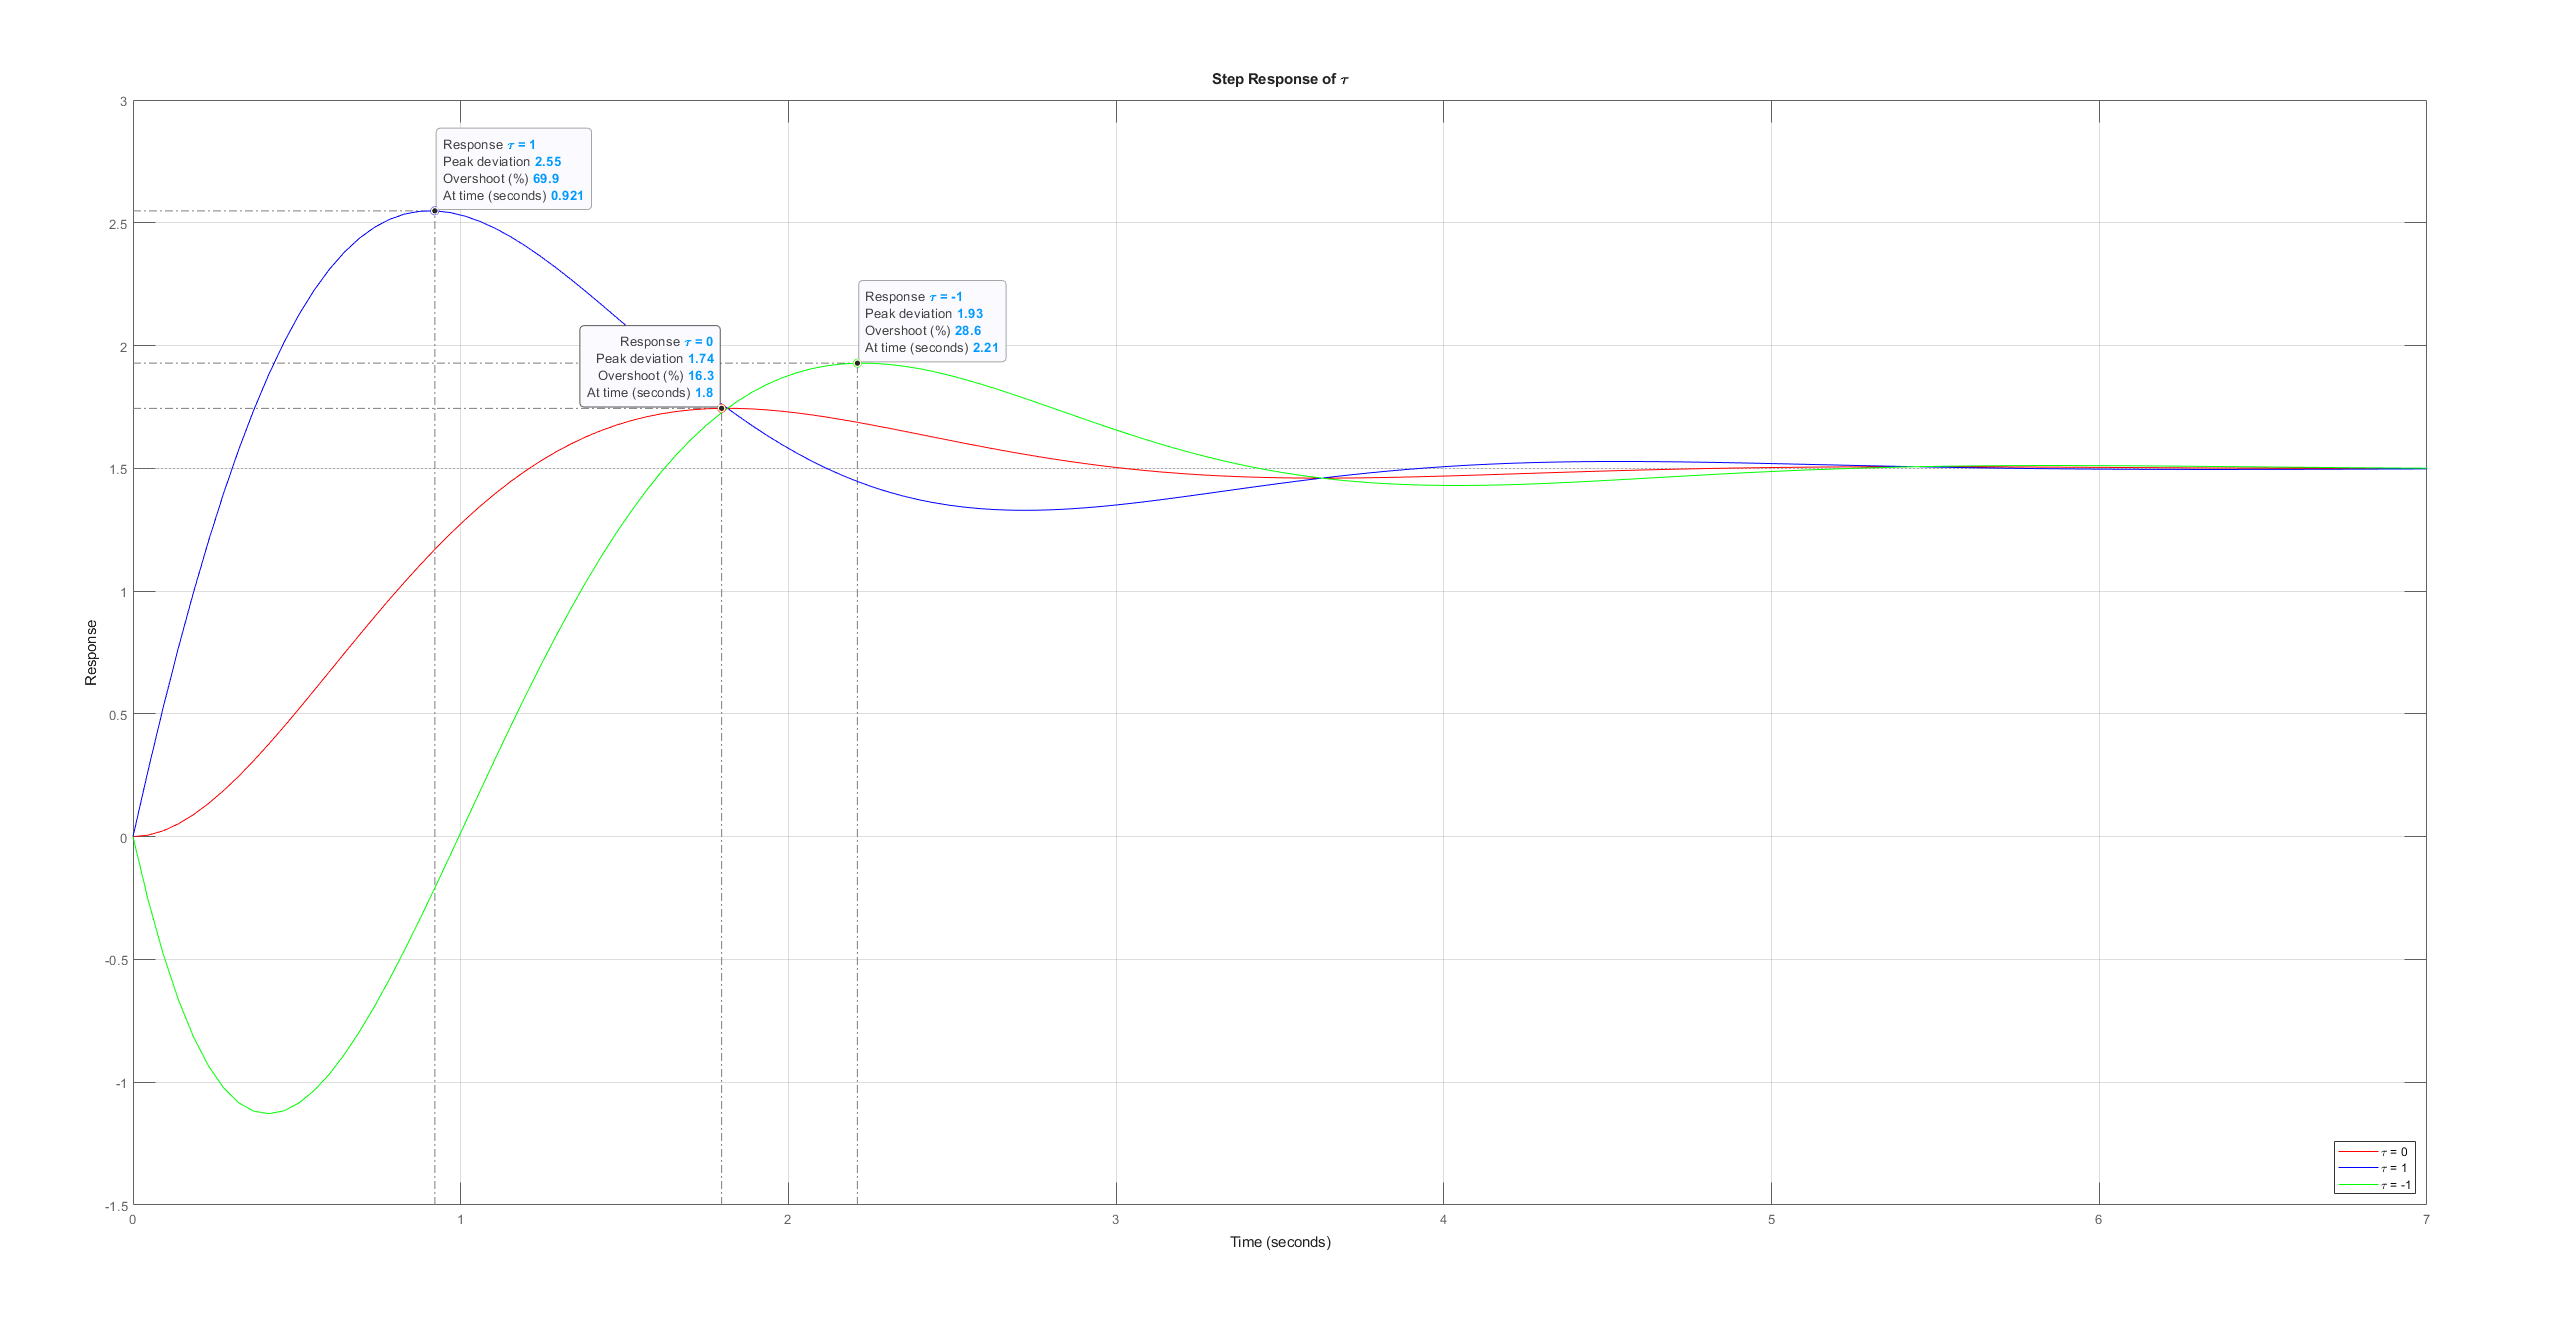
\includegraphics[width=\textwidth]{./images/s01a.png}
		\end{center}
		\caption{Step Response of \( \tau \) with labeled Peak Values and Times}\label{fig:s01a}
	\end{figure}

	\hwkPart{}

	When \( \tau = 0 \), the transfer function has no zeroes, and the response will be the same as the standard second-order response for complex conjugate poles. When \( \tau \neq 0 \), the zero of the transfer function will be \( z = \frac{-1}{\tau} \). Therefore, when \( \tau = -1 \), there is a zero in the LHP, and when \( \tau = 1 \), there is a zero in the RHP. As we discussed in class, the LHP zero will cause a higher peak overshoot and have a faster peak time compared to the standard second-order response. This behavior shows up in the plot, as seen with both \( \tau = 1 \) and \( \tau = -1 \).

	\lstinline{MATLAB} gives poles as \( -1 \pm 1.732j \).
	\begin{align*}
		t_{p} &= \frac{\pi}{\omega_{d}} \\
		      &= \frac{\pi}{1.732} \\
		t_{p} &= \qty{1.81}{\sec} \qed \\
		M_{p} &= e^{\sigma t_{p}} \\
		      &= e^{-1.81} = 0.16302 \\
		y_{p} &= \func{G}[0] \times \left(1+M_{p}\right) \\
		      &= \frac{3}{2} \left(1 + 0.16302\right) \\
		y_{p} &= 1.745 \qed
	\end{align*}
	
	These values align with the peak response and peak time given by \lstinline{MATLAB} for \( \tau = 0 \).

	\hwkCode{}

	\begin{lstlisting}[language={matlab}, label={lst:s01}, caption={\lstinline{MATLAB} code for P01}]
		s = tf('s');
		tau = [0, 1, -1];
		colors = ['r', 'b', 'g'];
		denom = s^2 + 2*s + 4;

		figure;
		hold on;
		for j = 1:length(tau)
			G = 6 * (tau(j) * s + 1) / denom;
			step(G,colors(j));
		end

		grid on;
		legend('\tau = 0', '\tau = 1', '\tau = -1', Location="southeast");
		title('Step Response of \tau');
		xlabel('Time');
		ylabel('Response');
		hold off;
	\end{lstlisting}

\end{hwkProblem}

\begin{hwkProblem}{2}{}

	\begin{enumerate}
		\item Repeat P01a if instead the denominator of \( \func{G}[s] \) is \( s^{2}+4s+4 \); label the settling times on the graph instead of the peaks
		\item For the \( \tau = 0 \) case, how does the settling time compare with the approximation discussed in the lecture? From the theory, would you expect to see any overshoot in the step response for this case?
		\item For the two cases where \( \tau \neq 0 \), do either exhibit overshoot? If so, how much? Is this overshoot associated with oscillations in the response?
	\end{enumerate}

	\hwkSol{}

	\hwkPart{}

	\begin{figure}[H]
		\begin{center}
			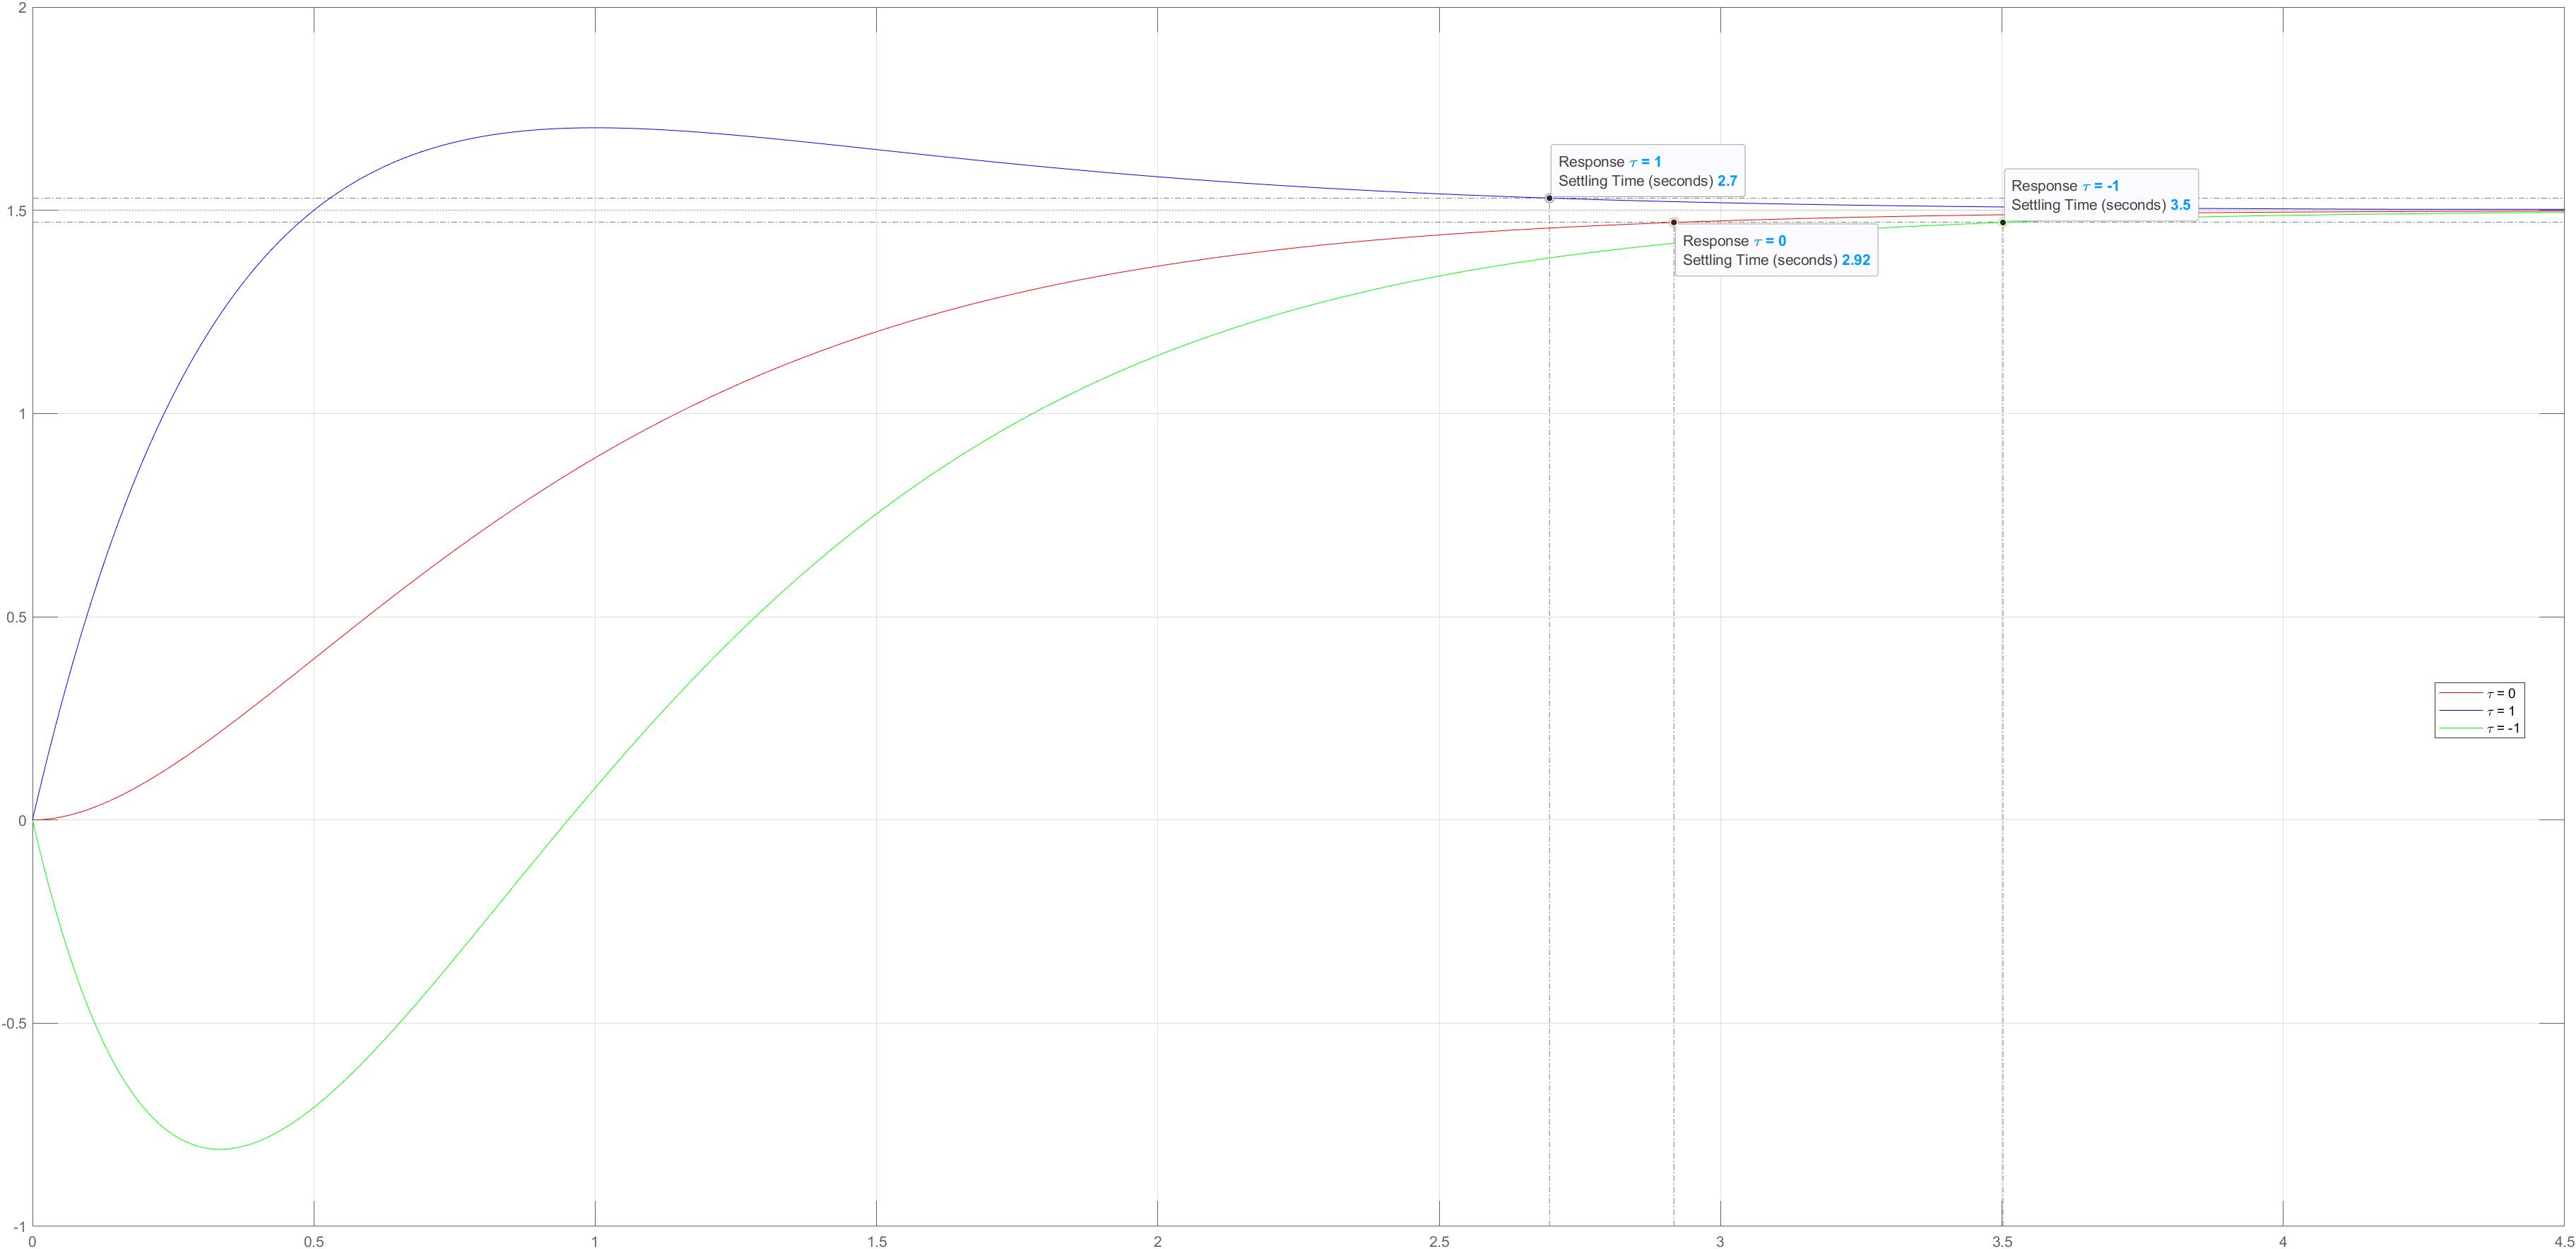
\includegraphics[width=\textwidth]{./images/s02a.png}
		\end{center}
		\caption{Step Response of \( \tau \) with labeled Settling Times}\label{fig:s02a}
	\end{figure}

	\hwkPart{}
	
	\lstinline{MATLAB} gives repeated poles of \( -2 \). For a repeated real pole, the damping ratio will be \( 1 \), and settling time will be \( \tau_{s} \approx \frac{6}{|\sigma|} = \qty{3}{\sec} \). \lstinline{MATLAB} gave a numerical settling time of \qty{2.92}{\sec}, which differs from the theoretical value we just found, and falls outside of the \qty{2}{\percent} approximation.

	As we discussed in class, when the transfer function has repeated real roots, the system response will not oscillate. Therefore, there will be no overshoot in the response, and will instead act like the standard first-order reponse.

	\hwkPart{}

	When \( \tau = 1 \), the system response overshoots, with a peak response of \( 1.7 \) (0.2 greater than the steady-state response). When \( \tau = -1 \), the system response undershoots. As stated in P02a, there will be no oscillations.

	\hwkCode{}

	\begin{lstlisting}[language={matlab}, label={lst:s02}, caption={\lstinline{MATLAB} code for P02}]
		denom = s^2 + 4*s + 4;

		figure;
		hold on;
		for j = 1:length(tau)
			G = 6 * (tau(j) * s + 1) / denom;
			step(G,colors(j));
		end

		grid on;
		legend('\tau = 0', '\tau = 1', '\tau = -1', 'Location', 'best');
		title('Step Response');
		xlabel('Time');
		ylabel('Response');
		hold off;
	\end{lstlisting}

\end{hwkProblem}

\begin{hwkProblem}{3}{}

	Use \lstinline{MATLAB} to obtain the Bode diagrams for the transfer function:
	\[
		\func{G}[s]=\frac{5000(s+0.02)}{3(2+s)(20+s)^{2}}
	\]
	\begin{enumerate}
		\item If the input to the system is \(\func{u}[t]=\sin(\frac{6 t}{10})\), what does the diagram predict the steady-state output of the system will be? Highlight the point(s) on each diagram you use to calculate this.
		\item Analytically verify your result in P03a by explicitly calculating \(\func{G}[\omega j],|\func{G}[\omega j]|\), and \(\angle \func{G}[\omega j]\) for the appropriate value of \(\omega\).
		\item If the input to the system is \(\func{u}[t]=2 \sin(70 t+\frac{\pi}{4})\), what do you expect the steady-state output of the system will be? Indicate the point(s) on each diagram you use to calculate this. Repeat P03b for this input.
		\item For an input of the form \(\func{u}[t]=2 \sin(\omega t)\), approximately what range of frequencies \(\omega\) would result in the largest amplitude oscillations in the steady-state output? Determine from the graph as exactly as possible the actual output amplitude at these frequencies. Verify using the technique in P03b.
		\item For the input in P03d, what value of \(\omega\) will result in the output oscillations lagging the input by \( \qty{90}{\degree} \) ("lag" = negative phase shift)? What will the amplitude of the output oscillations be at this frequency? Use the plot to estimate, then the technique in P03b for precision.
	\end{enumerate}

	\hwkSol{}

	\hwkPart{}

	With an input of \( \func{u}[t] = \sin(\frac{6 t}{10}) \), we take the points on the Bode Diagram corresponding to \( \omega = \qty{0.6}{\radian\per\sec} \).
	\begin{align*}
		\frac{A}{B} &= |\func{G}[\omega j]|,
		\begin{cases}
			A = |\func{G}[\omega j]| \\
			B = 1 \\
		\end{cases} \\
		\phi - \psi &= \angle \func{G}[\omega j],
		\begin{cases}
			\phi = \angle \func{G}[\omega j] \\
			\psi = 0 \\
		\end{cases} \\
		A &= |\func{G}[0.6j]| = \qty{1.65}{\decibel} \\
		  &= 10^{\frac{1.56}{20}} = 1.197 \\
		\phi &= \angle \func{G}[0.6j] = \qty{67.9}{\degree} = \qty{1.185}{\radian} \\
		y_{ss} &= 1.197 \sin(\frac{3}{5}t+1.185) \qed
	\end{align*}

	\begin{figure}[H]
		\begin{center}
			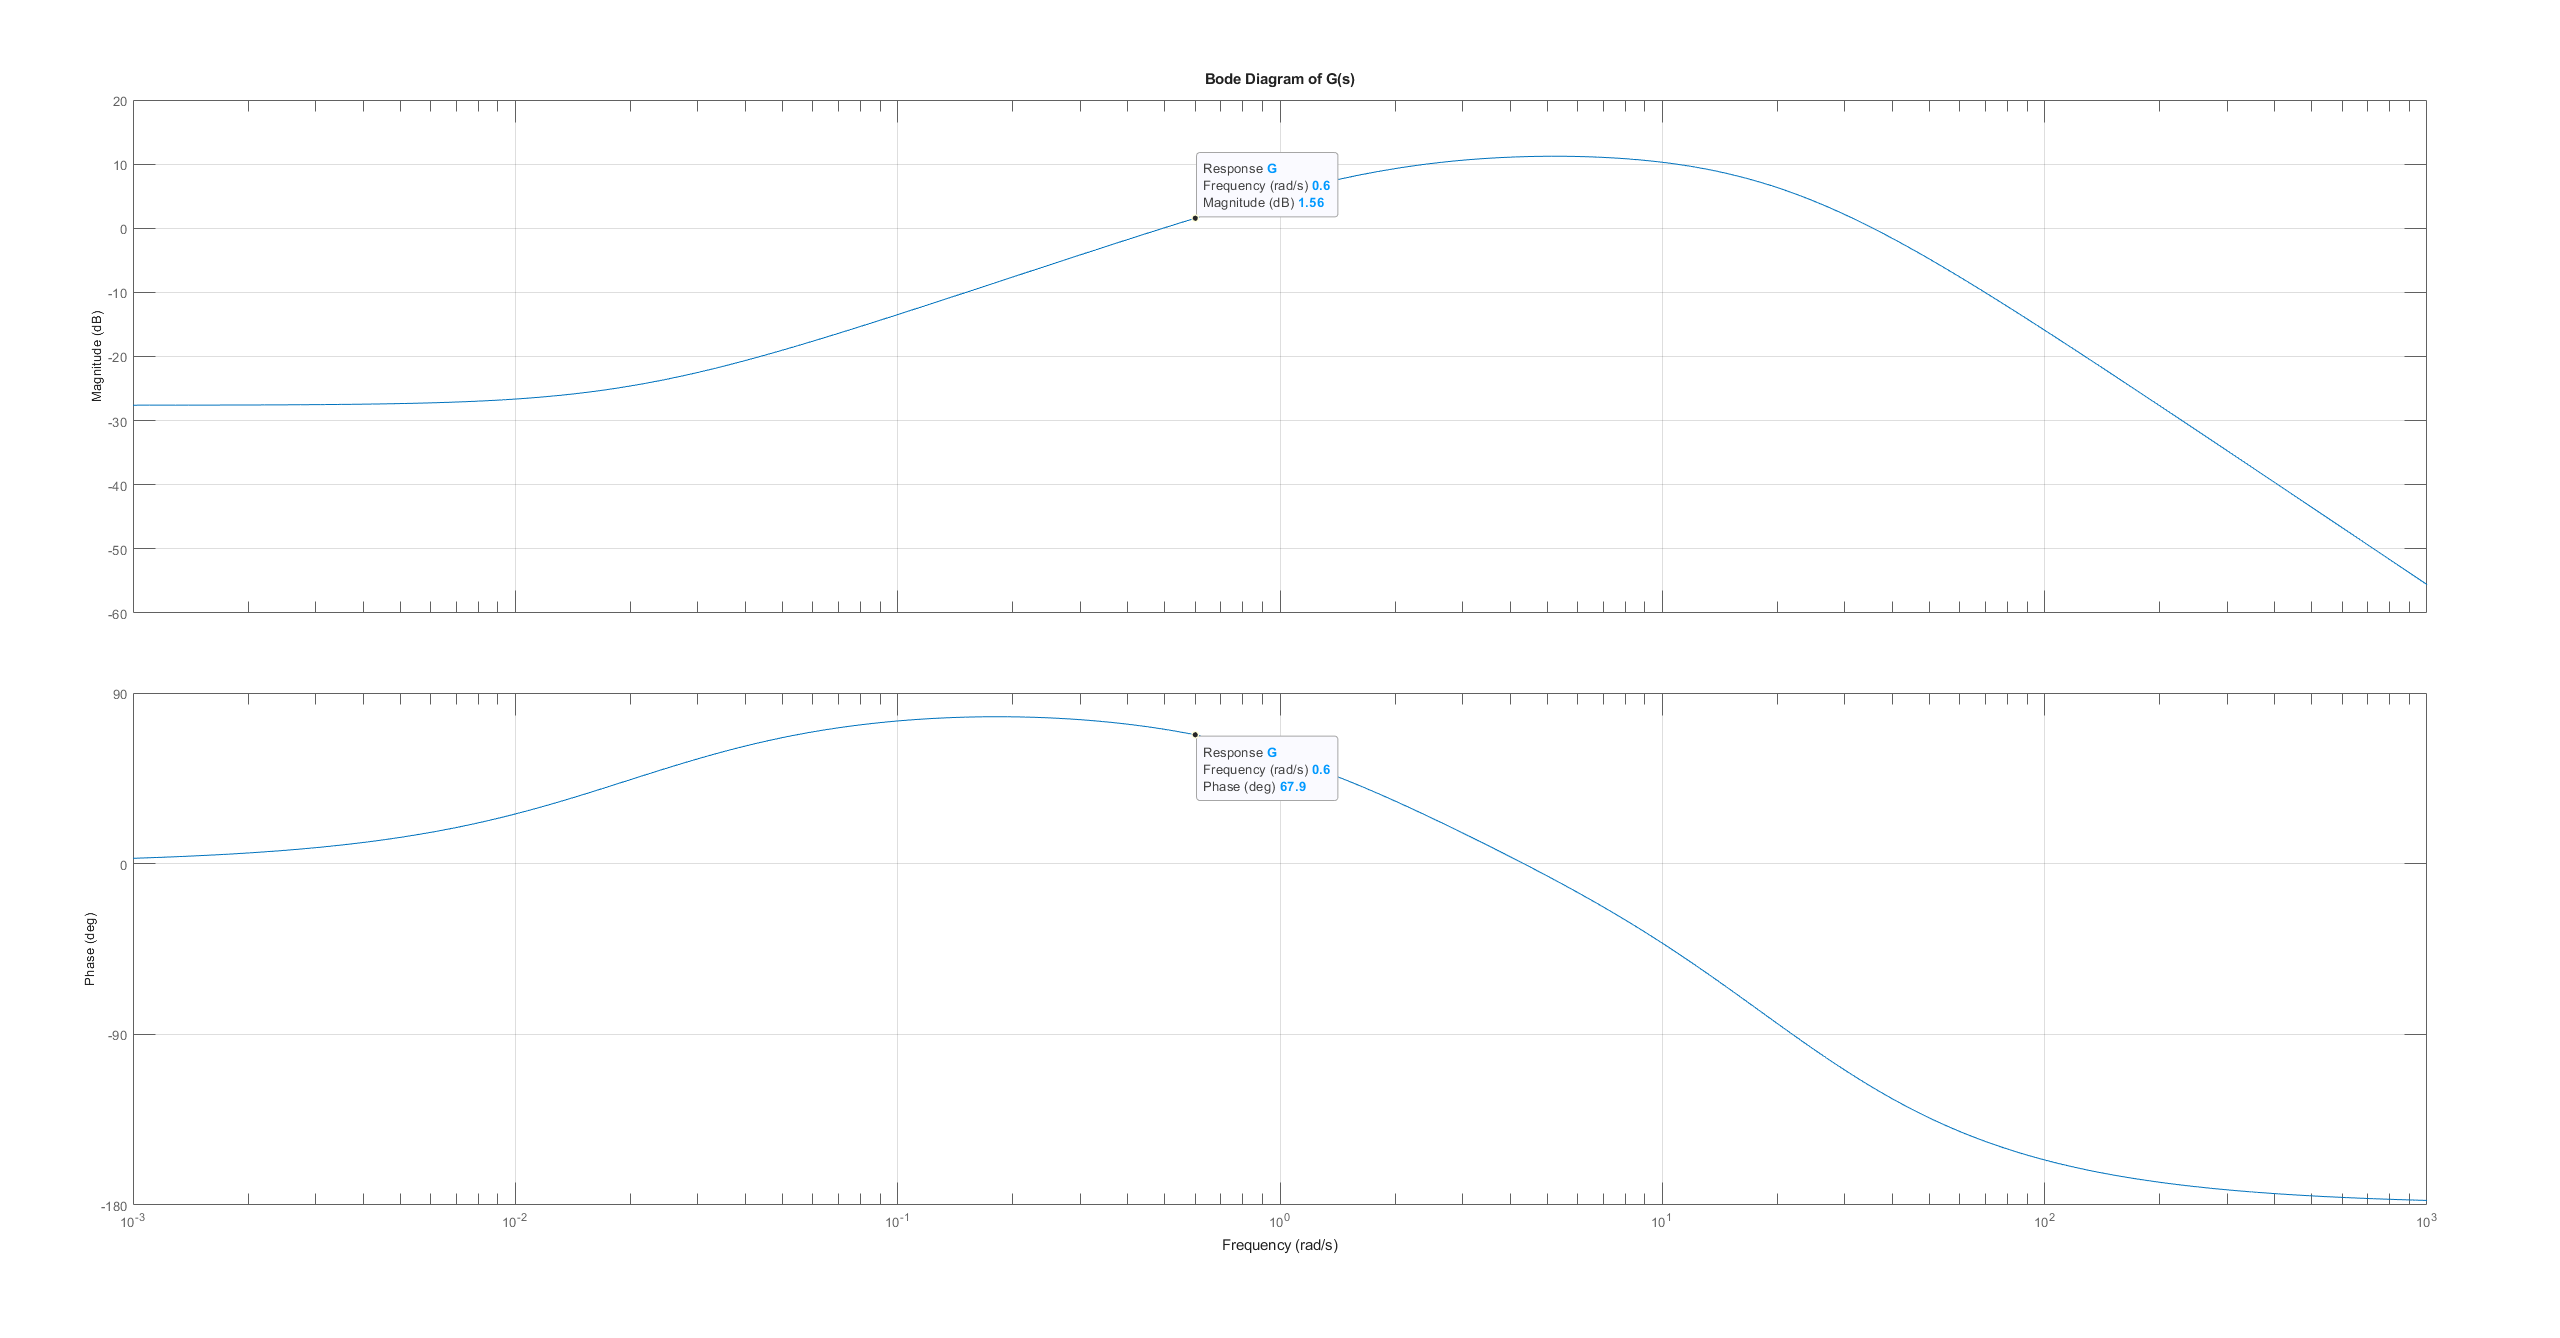
\includegraphics[width=\textwidth]{./images/s03a.png}
		\end{center}
		\caption{Bode Diagrams of \( \func{G}[s] \) with labeled Steady-State Locations}\label{fig:s03a}
	\end{figure}

	\hwkPart{}
	
	\begin{align*}
		\func{G}[0.6] &= \left. \frac{5000(s+0.02)}{3(2+s)(20+s)^{2}}\right|_{s=0.6} \\
		\func{G}[0.6] &= \frac{5000(s+0.02)}{3(2+0.6)(20+0.6)^{2}} = 0.4492 + 1.1094j \\
		|\func{G}[0.6]| &= \sqrt{\left(0.4492\right)^{2}+\left(1.1094\right)^{2}} = 1.197 \\
		\angle \func{G}[0.6] &= \tan^{-1}(\frac{1.1094}{0.4492}) = \qty{1.185}{\radian} \\
		y_{ss} &= 1.197 \sin(\frac{3}{5}t+1.185) \qed
	\end{align*}
	This result is the same as the one found in P03a.

	\hwkPart{}

	We repeat the same process as P03a and P03b, but with the points corresponding to \( \omega = \qty{70}{\radian\per\sec} \).
	
	Repeating P03a:
	\begin{align*}
		\frac{A}{B} &= |\func{G}[\omega j]|,
		\begin{cases}
			A = |\func{G}[\omega j]| \\
			B = 2 \\
		\end{cases} \\
		\phi - \psi &= \angle \func{G}[\omega j],
		\begin{cases}
			\phi = \angle \func{G}[\omega j] \\
			\psi = \frac{\pi}{4} \\
		\end{cases} \\
		|\func{G}[70j]| &= \qty{-10}{\decibel} \\
				&= 10^{\frac{-10}{20}} = 0.316 \\
		\angle \func{G}[70j] &= \qty{-146}{\degree} = \qty{-2.548}{\radian} \\
		A &= B |\func{G}[\omega j]| \\
		  &= 2 |\func{G}[70 j]| \\
		  &= 0.632 \\
		\phi &= \angle \func{G}[\omega j] + \psi \\
		     &= \angle \func{G}[70 j] + \frac{\pi}{4} \\
		     &= -2.548 + \frac{\pi}{4} = \qty{-1.762}{\radian} \\
		y_{ss} &= 0.632 \sin(70 t - 1.762) \qed
	\end{align*}
	Repeating P03b:
	\begin{align*}
		\func{G}[70j] &= \left. \frac{5000(s+0.02)}{3(2+s)(20+s)^{2}}\right|_{s=70j} \\
			      &= \frac{5000(70j+0.02)}{3(2+70j)(20+70j)^{2}} = -0.2621 - 0.1735j \\
		|\func{G}[70j]| &= \sqrt{\left(-0.2621\right)^{2}+\left(-0.1735\right)^{2}} = 0.314 \\
		\angle \func{G}[70j] &= \pi - \tan^{-1}(\frac{-0.1735}{0.2621}) = \qty{-2.557}{\radian} \\
		A &= B |\func{G}[\omega j]| \\
		  &= 2 |\func{G}[70 j]| \\
		  &= 0.628 \\
		\phi &= \angle \func{G}[\omega j] + \psi \\
		     &= \angle \func{G}[70 j] + \frac{\pi}{4} \\
		     &= -2.557 + \frac{\pi}{4} = \qty{-1.771}{\radian} \\
		y_{ss} &= 0.628 \sin(70 t - 1.771) \qed
	\end{align*}
	We get approximately the same answers from the Bode Diagram and numerical analysis.

	\begin{figure}[H]
		\begin{center}
			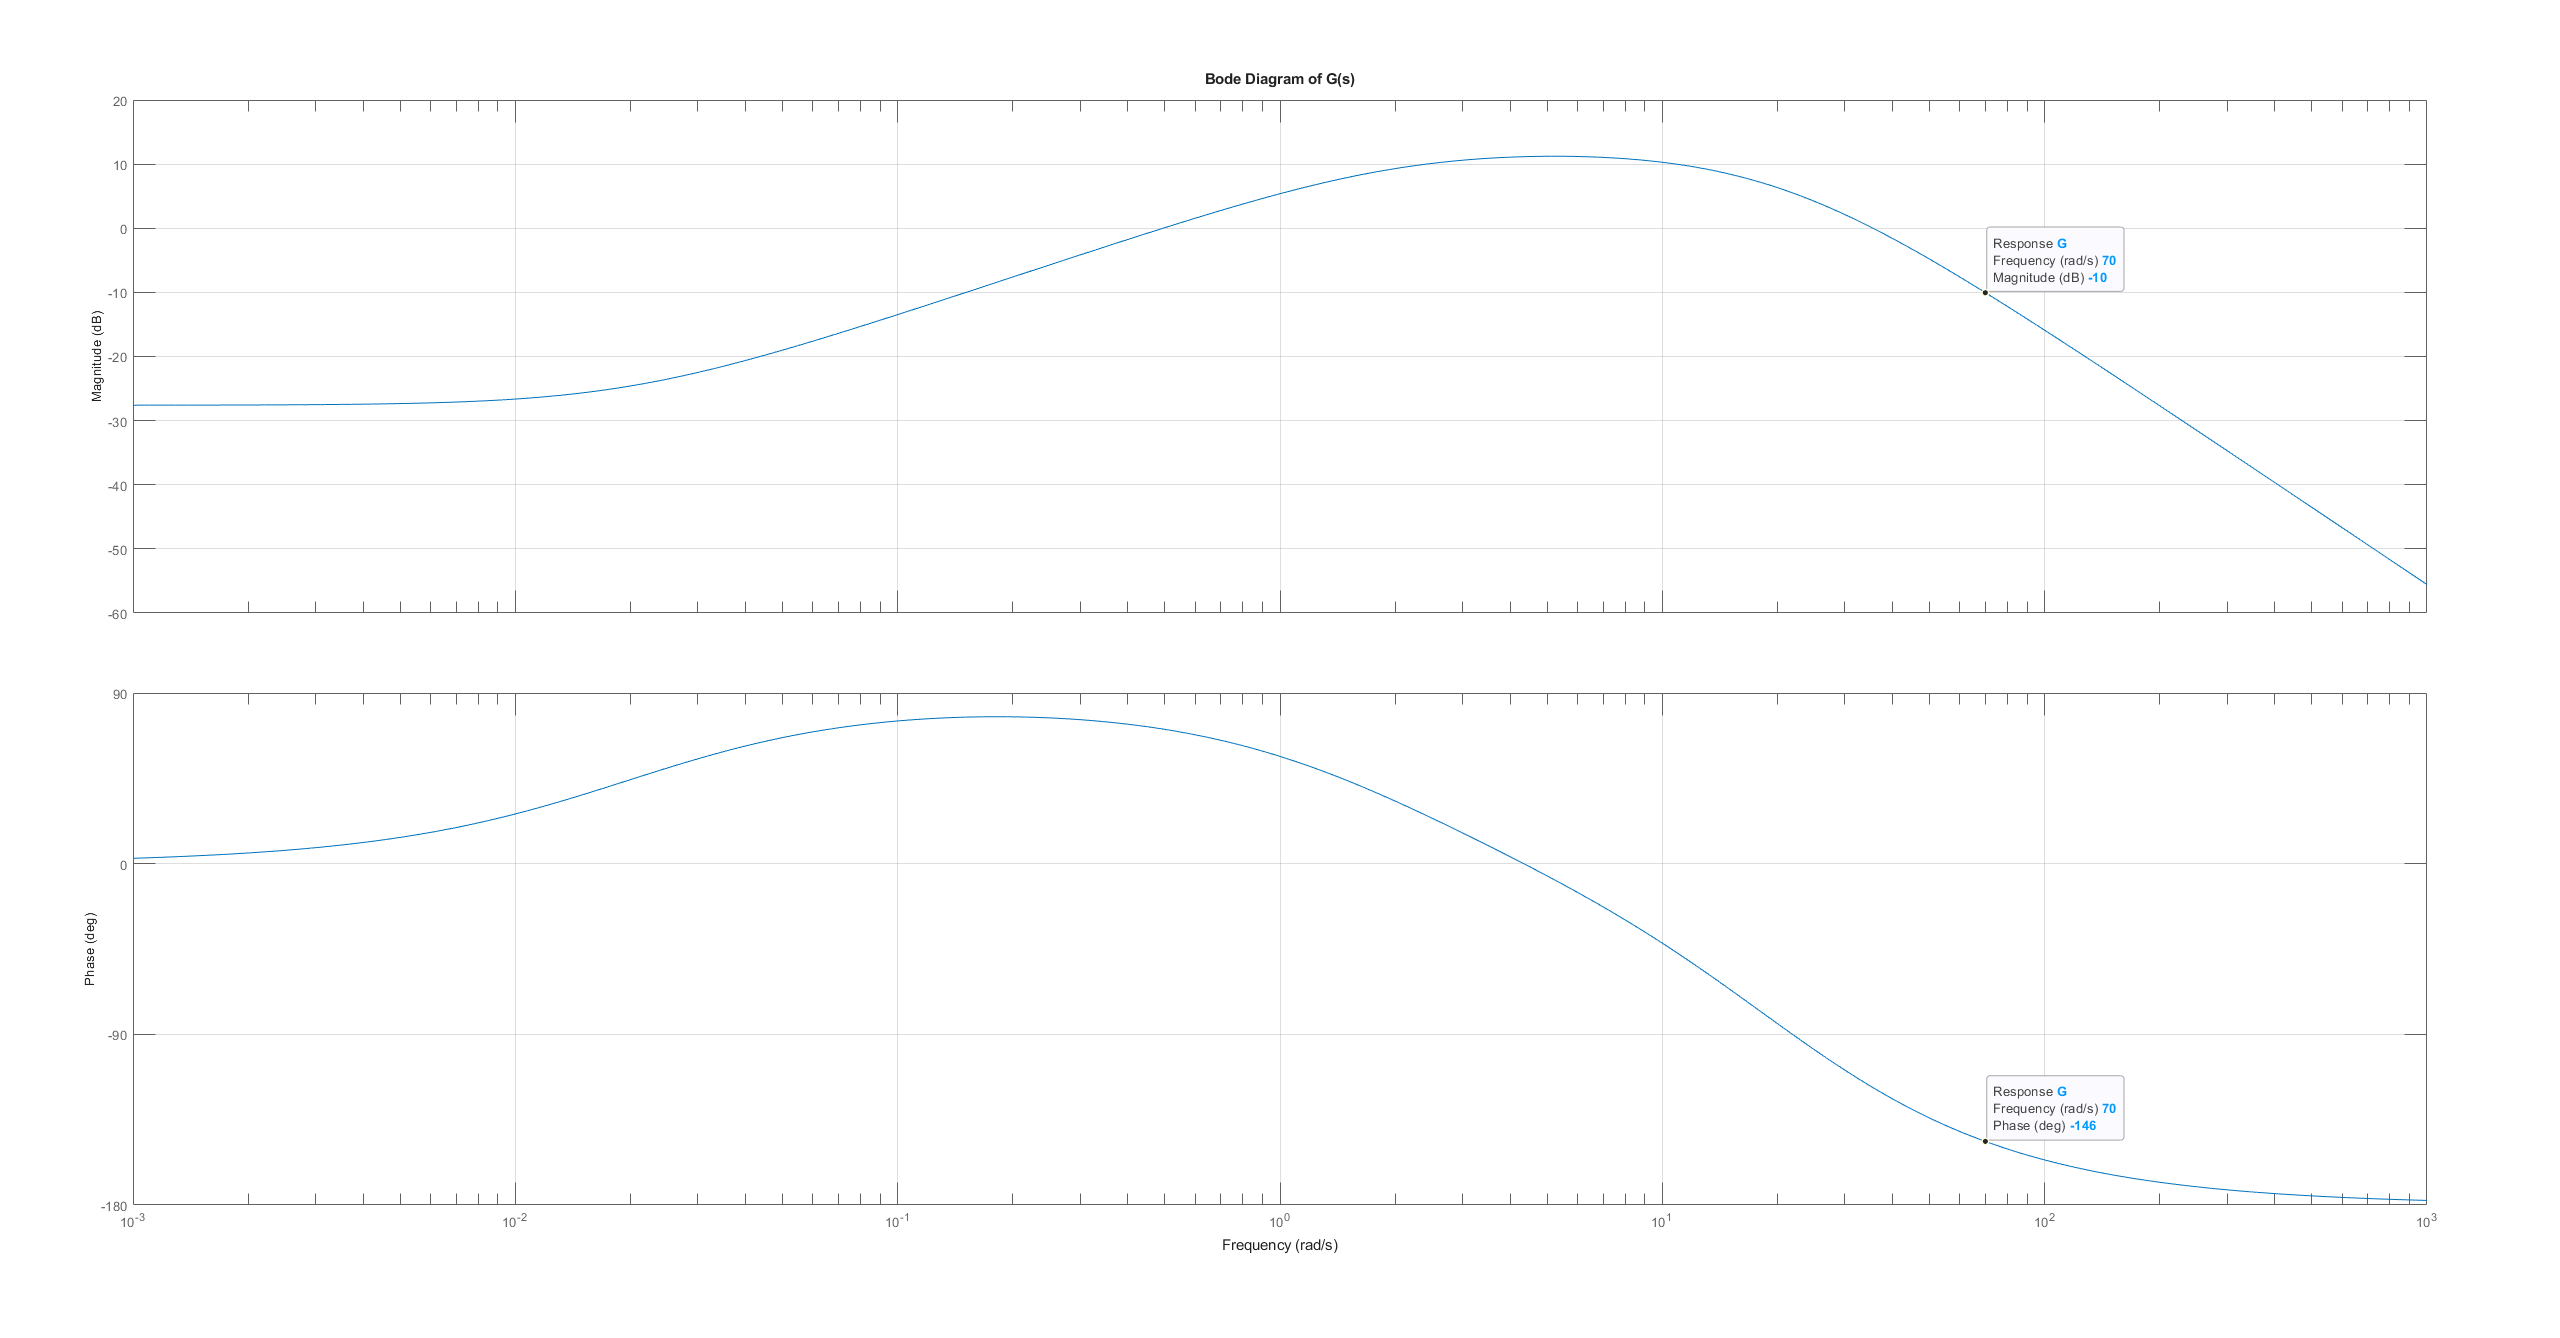
\includegraphics[width=\textwidth]{./images/s03c.png}
		\end{center}
		\caption{Bode Diagrams of \( \func{G}[s] \) with labeled Steady-State Locations}\label{fig:s03c}
	\end{figure}

	\hwkPart{}

	As \( A \) relies on \( |\func{G}[\omega j]| \) and \( B \), with constant \( B \), \( A \) (the amplitude of the steady-state oscillation) reaches its maximum when \( |\func{G}[\omega j]| \) is at its maximum. We can get this value from the Bode Diagram. \lstinline{MATLAB} gives this value as \qty{11.2}{\decibel} at \( \omega = \qty{5.22}{\radian\per\sec} \).
	\begin{align*}
		|\func{G}[5.22 j]| &= 10^{\frac{11.2}{20}} = 3.63 \\
		A &= B |\func{G}[\omega j]| \\
		  &= 2 |\func{G}[5.22 j]| \\
		A &= 7.26 \qed
	\end{align*}
	Verifying analytically:
	\begin{align*}
		\func{G}[5.22j] &= \left. \frac{5000(s+0.02)}{3(2+s)(20+s)^{2}}\right|_{s=5.22j} \\
			      &= \frac{5000(5.22j+0.02)}{3(2+5.22j)(20+5.22j)^{2}} = 3.603 - 0.539j \\
		|\func{G}[5.22j]| &= \sqrt{\left(3.603\right)^{2}+\left(-0.539\right)^{2}} = 3.643 \\
		A &= B |\func{G}[\omega j]| \\
		  &= 2 |\func{G}[5.22 j]| \\
		A &= 7.286 \qed
	\end{align*}
	We get approximately the same answers from the Bode Magnitude Diagram and numerical analysis, with a maximum amplitude of 7.3 at \( \omega = \qty{5.22}{\radian\per\sec} \).

	\hwkPart{}

	With an input of \( \func{u}[t] = 2\sin(\omega t) \), \( \psi = 0  \implies \phi = \angle \func{G}[\omega j] \). \lstinline{MATLAB} gives \( \angle \func{G}[\omega j] = \qty{-90}{\degree} \) when \( \omega = \qty{21.9}{\radian\per\sec} \). We now use the Bode Magnitude Diagram to find the amplitude at \( \omega = \qty{21.9}{\radian\per\sec} \) as \qty{5.52}{\decibel}.
	\begin{align*}
		|\func{G}[21.9 j]| &= 10^{\frac{5.52}{20}} = 1.888 \\
		A &= B |\func{G}[\omega j]| \\
		  &= 2 |\func{G}[21.9 j]| \\
		A &= 3.\bar{7} \qed
	\end{align*}
	Verifying analytically:
	\begin{align*}
		\func{G}[21.9j] &= \left. \frac{5000(s+0.02)}{3(2+s)(20+s)^{2}}\right|_{s=21.9j} \\
			      &= \frac{5000(21.9j+0.02)}{3(2+21.9j)(20+21.9j)^{2}} = -1.887 j \\
		|\func{G}[21.9j]| &= \sqrt{\left(-1.887\right)^{2}} = 1.887 \\
		A &= B |\func{G}[\omega j]| \\
		  &= 2 |\func{G}[21.9 j]| \\
		A &= 3.774 \qed
	\end{align*}
	We get approximately the same answers from the Bode Magnitude Diagram and numerical analysis, with an amplitude of 3.8 when there is \qty{90}{\degree} lag in the oscillations.

	\hwkCode{}

	\begin{lstlisting}[language={matlab}, label={lst:s03}, caption={\lstinline{MATLAB} code for P03}]
		G = (5000 * (s + 0.02))/(3 * (2 + s) * (20 + s)^2);
		w = logspace(-3, 3, 10000);
		figure;
		bode(G,w);
		grid on;
		title('Bode Diagram of G(s)');
	\end{lstlisting}

\end{hwkProblem}

\begin{hwkProblem}{4}{}

	\begin{enumerate}
		\item Give the Bode form for the transfer function in P03. Identify the Bode gain numerically. Discuss how and why this gain agrees with the "starting" (low frequency) magnitude shown on the left side of the Bode magnitude plot in P03.
		\item Use the \lstinline{bodemag} function in \lstinline{MATLAB} to get just the Bode magnitude diagram for the transfer function in P03, put a grid on it, and print out this plot (use \lstinline{orient landscape} just before printing to get a plot that fills the page horizontally). Sketch on top of this diagram the straight-line approximation using the technique described in class. Comment on the accuracy of this approximation.
	\end{enumerate}

	\hwkSol{}

	\hwkPart{}

	\begin{align*}
		N &= 0 \implies K_{B} = \func{G}[0] \\
		\func{G}[0] &= \left. \frac{5000(s+0.02)}{3(2+s)(20+s)^{2}}\right|_{s=0} \\
			    &= \frac{5000(0+0.02)}{3(2+0)(20+0)^{2}} = 0.0417 \\
		A_{\text{vdB}} &= 20 \log(K_{B}) \\
			       &= 20 \log(0.0417) \\
		A_{\text{vdB}} &= \qty{-27.6}{\decibel} \qed
	\end{align*}
	The Bode Gain for the transfer function is \qty{-27.6}{\decibel}, which agrees with the starting magnitude on the Bode Magnitude Diagram from \lstinline{MATLAB}. This is due to \( \omega \to 0 \) on the left axis of the plot, causing the transfer function to be approximately constant.

	\hwkPart{}

	The straight-line approximation is reasonably accurate, following the overall behavior pretty well. However, near the zeroes and the poles, the approximation fails, modeling the effects as sudden instead of gradual, creating sharp corners where there should be smooth curves.

	\begin{figure}[H]
		\begin{center}
			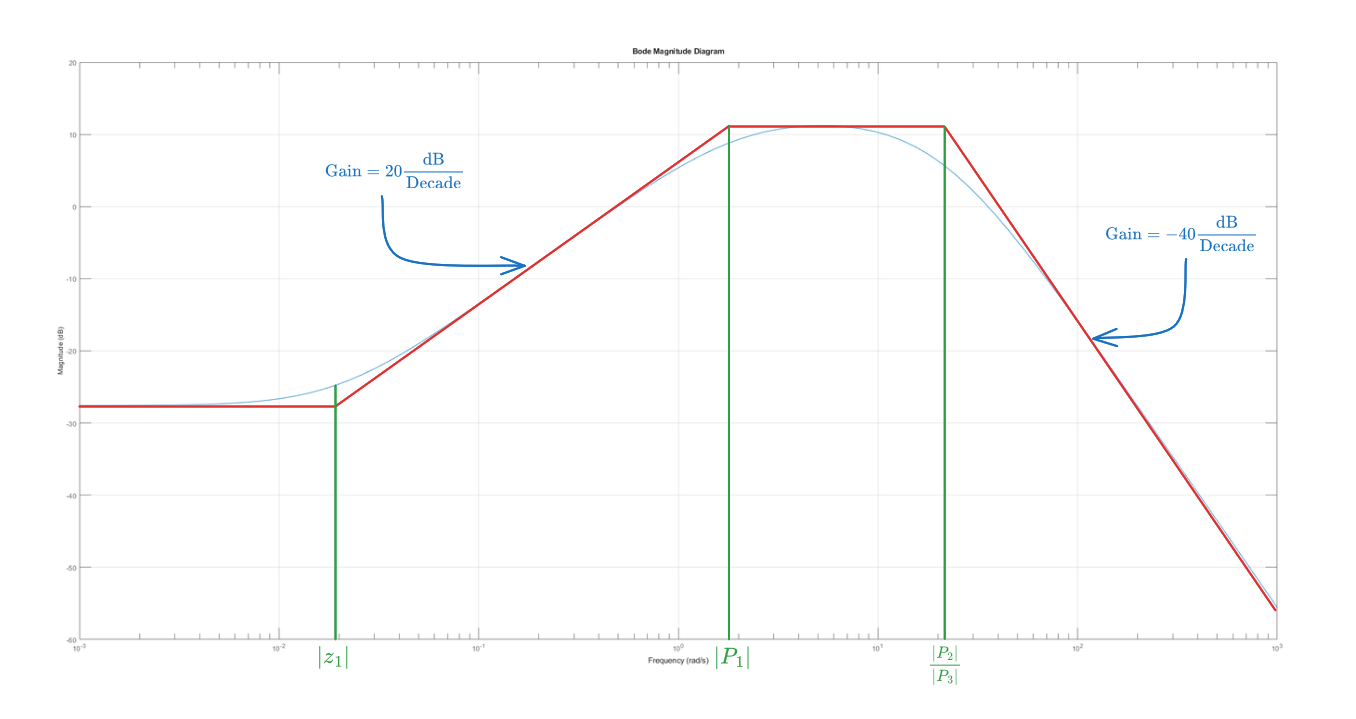
\includegraphics[width=\textwidth]{./images/s04b.png}
		\end{center}
		\caption{Bode Magnitude Diagram of \( \func{G}[s] \) with sketched Straight-Line Approximation}\label{fig:s04b}
	\end{figure}

	\hwkCode{}

	\begin{lstlisting}[language={matlab}, label={lst:s04}, caption={\lstinline{MATLAB} code for P04}]
		f1 = figure;
		bodemag(G);
		grid on;
		orient landscape;
		title('Bode Magnitude Diagram');
	\end{lstlisting}
	
\end{hwkProblem}

\end{document}
